
% ============================================================
% Supplementary Derivations for Information-Theoretic Analysis
% ============================================================


\subsection{Water-Filling Derivation}
\label{S4.1}
\subsection{Channel Capacity and the Water-Filling Solution}

The mutual information of Eq.~\ref{eq:mutual_info_cont} depends on the surface PSD $S_h(\mathbf{f})$, which is a property of the surface, not the instrument. The \textbf{channel capacity} $C$ is obtained by maximising mutual information over all possible surface spectra subject to a total power constraint:
\begin{equation}
    C = \max_{S_h(\mathbf{f}) \geq 0} \; \frac{A}{2} \iint \log_2\!\left[1 + \frac{|H(\mathbf{f})|^2 S_h(\mathbf{f})}{S_\eta(\mathbf{f})}\right] d^2\!f \quad \text{s.t.} \quad \iint S_h(\mathbf{f}) \, d^2\!f \leq \sigma^2
    \label{eq:capacity_max}
\end{equation}
where $\sigma^2$ is the total surface variance (power). This is a convex optimisation problem whose solution is the classical \textbf{water-filling} allocation~\cite{cover2006elements}:
\begin{equation}
    S_h^*(\mathbf{f}) = \max\!\left(0, \; \mu - \frac{S_\eta(\mathbf{f})}{|H(\mathbf{f})|^2}\right)
    \label{eq:waterfilling}
\end{equation}
where the ``water level'' $\mu$ is chosen to satisfy the power constraint. In $k$-space, the instrument should allocate more surface variance to frequencies where $|H(\mathbf{f})|^2 / S_\eta(\mathbf{f})$ is large---i.e., where the measurement is most informative.



\subsection{I-MMSE Identity}
\label{S4.2}
The relationship between MMSE and mutual information is governed by the \textbf{I-MMSE identity}~\cite{guo2005mutual}:
\begin{equation}
    \frac{d}{d\,\mathrm{snr}} I(h; y) = \frac{1}{2\ln 2} \cdot \mathrm{MMSE}(\mathrm{snr})
    \label{eq:immse}
\end{equation}
which establishes a fundamental duality: every bit of mutual information gained corresponds to a predictable reduction in MMSE. This identity has profound implications for surface metrology instrument design---it quantifies the exact trade-off between information throughput and reconstruction accuracy.

\begin{figure}[htbp]
    \centering
    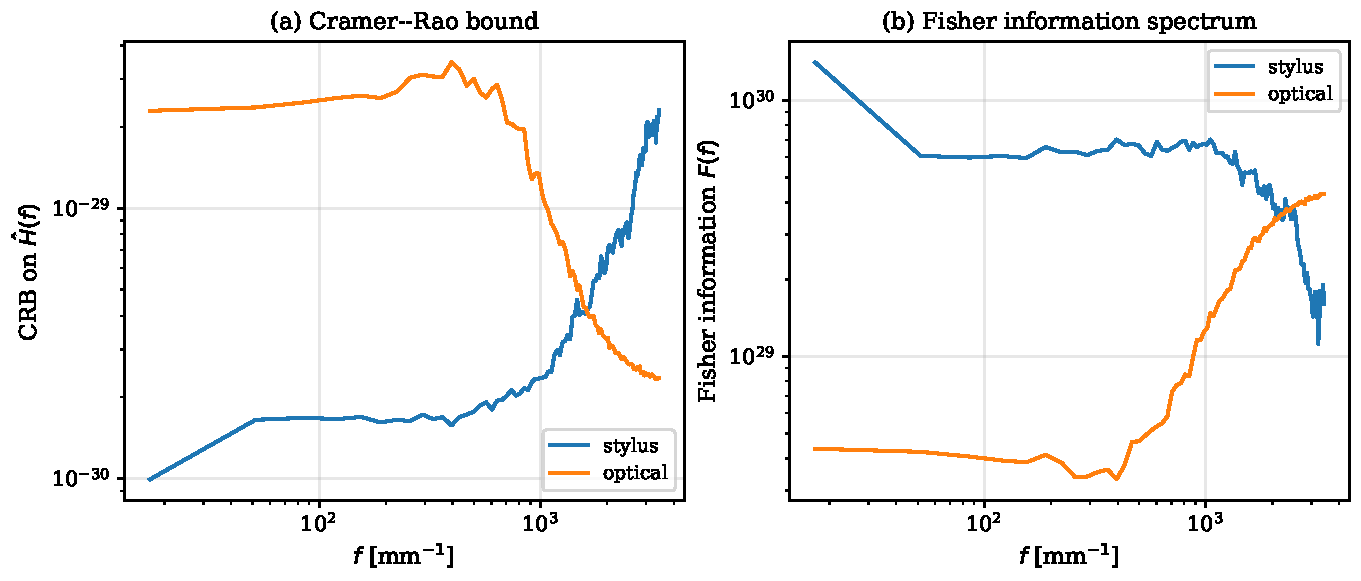
\includegraphics[width=\textwidth]{../pipeline/outputs/iter01/figures/fig8_cramer_rao.pdf}
    \caption{Cram\'{e}r--Rao uncertainty analysis. (a) The Cram\'{e}r--Rao uncertainty field $U(f_x,f_y)$ maps the minimum achievable estimation variance at each spatial frequency for both modalities; (b) comparison of the CRB-integrated uncertainty, showing that no signal processing algorithm can exceed these fundamental limits imposed by the instrument transfer function and noise characteristics.}
    \label{fig:cramer}
\end{figure}



\subsection{Information-Energy-Resolution Trilemma Derivation}
\label{S4.3}
\subsection{The Information--Energy--Resolution Trilemma}

The three fundamental resources in surface metrology are: (i) information extracted $I$, (ii) surface variance (``energy'') $\sigma^2$, and (iii) spatial resolution $\Delta x$. I show that these three quantities cannot be simultaneously optimised. The trade-off is governed by:
\begin{equation}
    I \cdot \frac{(\Delta x_\mathrm{eff})^2}{\sigma^2} \approx \frac{A}{2\ln 2} \cdot \frac{1}{\Delta f_\mathrm{eff}} \cdot \mathcal{F}(\overline{\mathrm{SNR}})
    \label{eq:trilemma}
\end{equation}
where $\mathcal{F}(\overline{\mathrm{SNR}})$ is a slowly varying function of the SNR. Equation~\ref{eq:trilemma} formalises the \textbf{Information--Energy--Resolution Trilemma}: for a fixed instrument and measurement area, increasing the extracted information $I$ requires either increasing the surface variance $\sigma^2$ (measuring rougher surfaces) or accepting coarser resolution $\Delta x_\mathrm{eff}$ (using a larger tip radius or lower NA). Conversely, achieving high resolution on a smooth surface necessarily yields less information.

For the baseline simulation: the trilemma product $I \cdot (\Delta x)^2 / \sigma^2$ equals $\num{2.0e21}$ for the stylus and $\num{3.4e21}$ for the optical system. The optical system's higher trilemma product indicates it makes more efficient use of the available surface ``energy'' to extract spatial information---a direct consequence of its broader transfer function sampling more of $k$-space per unit surface variance.


